\chapter{Implémentation et Réalisation}
\begin{spacing}{1.2}
\minitoc
\thispagestyle{MyStyle}
\end{spacing}
\newpage

\section{INTRODUCTION}
Ce chapitre présente les différentes étapes de la réalisation de notre projet de conversion d'images braille en texte lisible. Nous avons commencé par la description des ressources matérielles et logicielles utilisées. Ensuite, nous avons expliqué les détails de l'implémentation du modèle d'apprentissage automatique et de l'intégration des différentes étapes du projet.

\section{Environnement de Développement}
\subsection{Environnement matériel}
Notre projet a été implémenté sur un ordinateur portable dont les caractéristiques sont listées dans le tableau \ref{tab:caracteristiques}.

\begin{table}[H]
    \centering
    \begin{tabular}{|c|c|}
    \hline
    \textbf{Caractéristique} & \textbf{Détail} \\ \hline
    Marque & MSI \\ \hline
    Processeur & Intel(R) Core (TM) i5-11400H \\ \hline
    Mémoire & 8 GO \\ \hline
    Stockage & 512 GO SSD \\ \hline
    Système d'exploitation & Windows 10 Home \\ \hline
    \end{tabular}
    \caption{Caractéristiques de l'environnement matériel}
    \label{tab:caracteristiques}
\end{table}

\subsubsection{Environnement logiciel}
\paragraph{Google Colab}

Google Colab est un environnement de développement intégré basé sur le cloud, permettant de développer des scripts Python et d'exécuter des modèles d'apprentissage automatique avec TensorFlow. C'est un outil très utilisé pour les projets de traitement d'images, notamment grâce à sa compatibilité avec les GPU et TPU. Le logo de Google Colab est présenté à la figure \ref{fig:google_colab}.
\begin{figure}[H]
    \centering
    
\includegraphics[width=0.5\textwidth]{images/googlecolab.jpg}
    \caption{Logo de Google Colab}
    \label{fig:google_colab}
\end{figure}

\paragraph{TensorFlow}

TensorFlow est une bibliothèque open-source développée par Google pour le calcul numérique et l'apprentissage automatique. Elle permet d'implémenter des réseaux de neurones complexes pour le traitement des données d'image, comme celles du braille. Le logo de TensorFlow est présenté à la figure \ref{fig:tensorflow}.
\begin{figure}[H]
    \centering
    
\includegraphics[width=0.5\textwidth]{images/tensorflow.png}
    \caption{Logo de TensorFlow}
    \label{fig:tensorflow}
\end{figure}

\subsection{Langages de programmation, Frameworks et technologies utilisées}
\subsubsection{Python}
Python est le langage central utilisé dans notre projet. C’est un langage de programmation polyvalent, particulièrement adapté pour le développement de solutions en apprentissage automatique. Il a été utilisé pour manipuler notre dataset et développer les réseaux neuronaux avec TensorFlow. Le logo de Python est présenté dans la figure \ref{fig:python}.
\begin{figure}[H]
    \centering
    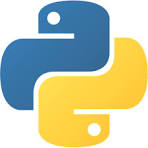
\includegraphics[width=0.5\textwidth]{images/Logo de Python.jpg}
    \caption{Logo de Python}
    \label{fig:python}
\end{figure}

\subsubsection{Keras}
Keras est une API de haut niveau construite sur TensorFlow, qui a facilité la construction et l'entraînement de notre modèle de deep learning. Elle est particulièrement utilisée pour la création rapide de prototypes et l'expérimentation avec différents modèles de réseaux neuronaux. Le logo de Keras est illustré à la figure \ref{fig:keras}.
\begin{figure}[H]
    \centering
    
\includegraphics[width=0.5\textwidth]{images/keraslogo .png}
    \caption{Logo de Keras}
    \label{fig:keras}
\end{figure}

\section{Implémentation du Modèle de Reconnaissance de Braille}

\subsection{Prétraitement des Données}
Avant d'entraîner le modèle, nous avons effectué plusieurs étapes de prétraitement :
1. **Chargement et Redimensionnement** : Les images de braille ont été chargées et redimensionnées à une taille uniforme pour garantir une homogénéité dans le modèle.
2. **Normalisation des Pixels** : Les valeurs des pixels ont été normalisées entre 0 et 1 pour faciliter l'apprentissage du modèle.

\subsection{Création du Modèle}
Nous avons construit un modèle de réseau de neurones convolutifs (CNN) en utilisant Keras, qui est adapté pour traiter des images. La structure du modèle a inclus plusieurs couches de convolution, suivies de couches de pooling et de couches denses. Cette approche a permis d'extraire des caractéristiques pertinentes des images de braille.

\subsection{Entraînement du Modèle}
Le modèle a été entraîné à l'aide de notre dataset d'images de braille. Nous avons utilisé la fonction de perte appropriée et l'optimiseur Adam pour optimiser l'apprentissage. Des techniques de data augmentation ont été mises en place pour améliorer la robustesse du modèle face aux variations d'éclairage et d'orientation des images.

\subsection{Évaluation et Validation}
Après l'entraînement, le modèle a été évalué sur un ensemble de validation afin de mesurer sa précision. Nous avons également tracé des courbes d'apprentissage pour analyser le surapprentissage et ajuster les hyperparamètres.

\subsection{Intégration avec l'Application Mobile}
Enfin, le modèle a été intégré dans une application mobile développée avec Xamarin Forms, permettant aux utilisateurs de prendre des photos d'images de braille, qui sont ensuite traitées par le modèle pour afficher le texte correspondant. Cette intégration a nécessité des ajustements pour garantir une expérience utilisateur fluide.

\section{Conclusion}
En résumé, ce chapitre a exposé le processus d'implémentation de notre modèle de reconnaissance de braille, de l'environnement de développement à l'intégration finale. Chaque étape a été cruciale pour garantir le succès du projet et fournir une solution fonctionnelle qui répond aux besoins des utilisateurs.
